\documentclass[
hyperref={pdfpagelabels=false}
%,red %, notes=show
,xcolor=table
% ,handout % UNCOMMENT FOR HANDOUT - also uncomment \pgfpagesuselayout
]
{beamer}

%\usecolortheme{beaver}


\setlength {\marginparwidth }{2cm}
\usepackage{todonotes}

\definecolor{Myred}{rgb}{0.7, 0.2, 0.2}

\usecolortheme[named=Myred]{structure}


\usepackage{pres}
% \usepackage{mathdots}
%\usepackage{qtree}
\usepackage{pgfpages}
% \pgfpagesuselayout{4 on 1}[a4paper, landscape,border shrink=5mm]
%\pgfpagesuselayout{2 on 1}[a4paper,border shrink=5mm]
\pgfpageslogicalpageoptions{1}{border code=\pgfusepath{stroke}}
\pgfpageslogicalpageoptions{2}{border code=\pgfusepath{stroke}}
\pgfpageslogicalpageoptions{3}{border code=\pgfusepath{stroke}}
\pgfpageslogicalpageoptions{4}{border code=\pgfusepath{stroke}}

\usepackage{picture}
\usepackage{pgfplots}
\usepackage{filecontents}
% \pgfplotsset{compat=1.12}
\usepackage{pdflscape}

\beamertemplatenavigationsymbolsempty

\newcommand{\travail}{\textbf{ICI IL Y A D TRAVAIL!}}

%%%%%%%%%%%%%%%%%%%%%%%%%%%%%
%%%%% PRESENTATION INFO %%%%%
%%%%%%%%%%%%%%%%%%%%%%%%%%%%%
\title[CSC - Intro]{Secured Communication Protocols \\ --Cryptographie et Sécurité des Communications--} 
\author[]{Lionel Morel}
\institute[]{Telecommunications - INSA Lyon}
\date{Fall-Winter 2021-22}


%%%%%%%%%%%%%%%%%%%%%%%%%
%%%%%%%% COLORS %%%%%%%%%
%%%%%%%%%%%%%%%%%%%%%%%%%
\definecolor{greenCiti}{RGB}{83,186,89}
\definecolor{darkGreen}{RGB}{60,132,136}
\definecolor{purple}{RGB}{76, 69, 164}
\colorlet{corecolor}{lightgray}
\definecolor{uncorecolor}{RGB}{222,181,182}
\definecolor{lightgray}{rgb}{0.8,0.8,0.8}
\definecolor{lightblue}{RGB}{188,212,244}
\colorlet{socketcolor}{blue!20}

\colorlet{getpcolor}{red}
\colorlet{leetcolor}{darkGreen}

\definecolor{redfixit}{RGB}{188,43,0}
\definecolor{yellowfixit}{RGB}{235,237,62}
\definecolor{bluefixit}{RGB}{7,2,236}
\definecolor{orangefixit}{RGB}{227,118,24}
\definecolor{cyanfixit}{RGB}{1,171,159}
\definecolor{purplefixit}{RGB}{206,92,232}
\definecolor{greenfixit}{RGB}{102,156,52}



\begin{document}

\begin{frame}
  \maketitle
\end{frame}

\section{Context}


\begin{frame}
  \frametitle{Symmetric Cryptography}

  \begin{center}
    \includegraphics[width=\textwidth]{symCrypto-basic.pdf}
  \end{center}

  \begin{itemize}
  \item Encryption/Decryption is cheap
  \item State-of-the-Art: AES
  \item Limitation: requires a key-sharing mechanism
  \end{itemize}
  
\end{frame}


\begin{frame}
  \frametitle{Diffie-Hellman Key Exchange}
  \begin{center}
    \includegraphics[width=\textwidth,height=0.7\textheight,keepaspectratio]{fig/DiffieHellman.pdf}
  \end{center}
\end{frame}


\begin{frame}
  \frametitle{Asymmetric Cryptography}

  \begin{itemize}
  \item Each participant builds a $(Pub_k, Priv_k)$ pair of keys
  \end{itemize}

\
  
  \begin{minipage}[t]{.45\textwidth}
    \textbf{Encryption}
    
    \includegraphics[width=\textwidth,height=0.6\textheight,keepaspectratio]{fig/RSA-encryption.pdf}
  \end{minipage}
  \hfill
  \begin{minipage}[t]{.45\textwidth}
   \textbf{Decryption}

   \includegraphics[width=\textwidth,height=0.6\textheight,keepaspectratio]{fig/RSA-decryption.pdf}
  \end{minipage}
  
\end{frame}


\begin{frame}
  \frametitle{Message-Authentication-Codes (hashes)}

  \begin{center}
    \includegraphics[width=\textwidth]{hmac.pdf}
  \end{center}
\end{frame}


\begin{frame}
  \frametitle{Self-signed Certificates}

  \begin{minipage}[t]{.45\linewidth}
    \textbf{Sign}
    
    \includegraphics[width=\textwidth]{self-signed-certificates.pdf}        
  \end{minipage}
  \hfill
  \begin{minipage}[t]{.45\linewidth}
    \textbf{Verify}
    
    \includegraphics[width=\textwidth]{self-signed-certificates_check.pdf}    
  \end{minipage}

  \begin{itemize}
  \item Problem: Man-in-the-Middle
  \end{itemize}
  
\end{frame}

\begin{frame}
  \frametitle{Man-in-the-Middle}

  \begin{itemize}
  \item Bob and Alice want to communicate
  \item Bob $\longrightarrow$ \fbox{$(B,Pub_B)$} $\longrightarrow$ Alice
  \item Hypothesis: Charlie can read and modify messages between Bob and Alice. 
  \item Charlie falsifies Key definition of Bob: \\
    Bob $\longrightarrow$ \fbox{$(B,Pub_B)$} $\longrightarrow$ Charlie $\longrightarrow$ \fbox{$(B,Pub_C)$} $\longrightarrow$ Alice\\
    (he also keeps $Pub_B$ for later)
  \item Now when Alice writes to Bob, she actually uses Charlie's public key
  \item Alice $\longrightarrow$ \fbox{$\{m\}_{Pub_C}$} $\longrightarrow$ Bob
  \item Charlie can then eavesdrop all messages:\\
    Alice $\longrightarrow$ \fbox{$\{m\}_{Pub_C}$} $\longrightarrow$ Charlie $\rightarrow$ $\{\{m\}_{Pub_C}\}_{Priv_C} = m$ $\longrightarrow$ \fbox{$\{m\}_{Pub_B}$} $\longrightarrow$ Bob
  \end{itemize}
  
\end{frame}




\begin{frame}
  \frametitle{Public-Key Infrastructure and Certificate Authorities}
  A PKI consists of: 
  \begin{itemize}
  \item A \textbf{Certificate Authority} (CA) - stores, issues and signs digital certificates
  \item A \textbf{Registrtion Authority} (RA) - verifies identity of entities requesting their certificates to be stored at the CA. 
  \item A \textbf{Central Directory} - secure location to store keys 
  \end{itemize}

  \begin{itemize}
  \item CAs are ``Trusted Third Party''
  \end{itemize}

  
\end{frame}


% \begin{frame}
%   \frametitle{Certificate Authorities}
%   \begin{itemize}
%   \item 
%   \end{itemize}
% \end{frame}


% \begin{frame}
%   \frametitle{DANE}
% \end{frame}


% \begin{frame}
%   \frametitle{PGP}
% \end{frame}



\begin{frame}
  \frametitle{TLS}
  \begin{itemize}
  \item History:
    \begin{itemize}
    \item SSL proposed in 1995 by Netscape (RIP)
    \item TLS proposed by the IETF, starting 1999
    \item Current version 1.3 (2018)
    \end{itemize}
  \item TLS stands for Transport Layer Security
  \item It supercedes SSL 
  \item Works on top of TCP/IP
  \item Application-indenpendant, etg: HTTPs = HTTP+TLS, IMAPS = IMAP+TLS
  \end{itemize}
\end{frame}

\begin{frame}
  \frametitle{TLS (cont'd)}

  \textbf{Confidentiality}
  \begin{itemize}
  \item Exchanged data is encrypted using \textbf{Symmetric-key cryptography}
  \item Encryption keys are re-newed for every session, ie TLS uses \textbf{session keys}
  \end{itemize}

  \textbf{Authenticity}
  \begin{itemize}
  \item Identity of communicating parties is authenticated using \textbf{Public-key cryptography}
  \end{itemize}

  \textbf{Integrity}
  \begin{itemize}
  \item Each message includes a \textbf{Message Authentication Code} to prevent alteration
  \end{itemize}
\end{frame}


\begin{frame}
  \frametitle{TLS (cont'd)}

  \begin{itemize}
  \item Client and server \textbf{agree to use TLS}
  \item They perform a \textbf{handshare procedure} together (see next)
  \item Out of this handshake, they get (secret) encryption keys they can then use to perform \textbf{symmetric encryption}
  \end{itemize}
 
\end{frame}


\begin{frame}
  \frametitle{TLS handshake}

  \begin{center}
    \includegraphics[scale=0.7]{TLS-handshake.pdf}
  \end{center}

\end{frame}


\begin{frame}
  \frametitle{SSH}
  \begin{itemize}
  \item SSH stands for Secured Shell
  \item Provides a way to connect (shell) to a distant computer while encrypting all data exchanged
  \item Before SSH:
    \begin{itemize}
    \item data was sent unencrypted over the network
    \item not so bad as internet was not there :) 
    \end{itemize}
  \item 1995: Tatu Ylönen proposed a secured version of a remote shell
  \end{itemize}
\end{frame}

\begin{frame}
  \frametitle{Sending Data Through SSH}
  \begin{itemize}
  \item Consider a TCP connexion between 2 machines
  \item SSH breaks data into a series of packets
  \end{itemize}

  \begin{center}
    \includegraphics[width=0.7\textwidth]{ssh-packet.pdf}
  \end{center}

  {\scriptsize   \textbf{Algorithms available}
    \begin{itemize}
    \item EdDSA, ECDSA, RSA and DSA for public-key cryptography.
    \item ECDH and Diffie–Hellman for key exchange.
    \item HMAC, AEAD and UMAC for MAC.
    \item AES (and deprecated RC4, 3DES, DES[29]) for symmetric encryption.
    \item AES-GCM] and ChaCha20-Poly1305 for AEAD encryption.
    \item SHA (and deprecated MD5) for key fingerprint.
    \end{itemize}
  }
\end{frame}

\begin{frame}
  \frametitle{SSH properties}
  \begin{itemize}
  \item Channel multiplexing: You can open a number of different channels to send different
    data to/from different partners
  \item Tunneling: on can redirect a (eg) TCP flow into an ssh tunnel 
  \item Distant shell
  \item File transfer
  \item Port redirection
  \end{itemize}
\end{frame}


\begin{frame}
  \frametitle{SSH Authentication}
  \begin{block}{Client-side}
  \begin{itemize}
  \item password
  \item public/private key
  \end{itemize}
\end{block}

\begin{block}{Server-side}
  \begin{itemize}
  \item at 1st connection, server stores client's key footprint
  \item for follow-up connection, server checks footprint
  \item if key is invalid: connection refused
  \end{itemize}
\end{block}

\begin{block}{NB}
  No guarantee on 1st connection $\Longrightarrow$ ``\textit{opportunistic security}''
\end{block}
\end{frame}


\begin{frame}
  \frametitle{OpenSSH}
  OpenSSH is a software suite that includes command-line utilities and daemons:
  \begin{itemize}
  \item \texttt{scp} (replacement for \texttt{rcp}) to copy files through encryted channel
  \item \texttt{sftp}, replacement for \texttt{ftp}
  \item \texttt{ssh} itself
  \item \texttt{ssh-agent} to hold keys and ease authentication
  \item \texttt{ssh-keygen} to generate RSA, DSA or elliptic-curve keys
  \item \texttt{sshd} the ssh server daemon
  \end{itemize}
\end{frame}


\begin{frame}
  \frametitle{Needham-Schroeder Symmetric Protocol (1978)}

  \begin{itemize}
  \item A and B want to talk
  \item A (resp B) has a private key with server S, $k_{AS}$ (resp $k_{BS}$)
  \end{itemize}

  
  \begin{center}
    \includegraphics[width=0.9\textwidth]{needham-shcroeder-symm.pdf}
  \end{center}

  NB: Vulnerable to replay attack: 
  \begin{itemize}
  \item Charlie gets an old compromised key $K_{AB}$ and pretends to be A by sending $\{K_{AB}, A\}_{K_{BS}}$ to B
  \end{itemize}
\end{frame}



\begin{frame}
  \frametitle{Needham-Schroeder: fixing the Replay Attack}

  \begin{center}
    \includegraphics[width=0.9\textwidth]{needham-shcroeder-symm-replay-fix.pdf}
  \end{center}
\end{frame}



\begin{frame}
  \frametitle{Needham-Schroeder Public-Key Protocol}

  A: $(k_{PA}, k_{SA})$    B: $(k_{PB}, k_{SB})$      S: $(k_{PS}, k_{SS})$  


  \begin{center}
    \includegraphics[width=0.9\textwidth]{needham-shcroeder-asym.pdf}
  \end{center}  
  
\end{frame}



\begin{frame}
  \frametitle{Kerberos}
  \begin{itemize}
  \item Active Directory's main authentication protocol
  \item No public key (symmetric keys only)
  \item How to share keys ?
    \begin{itemize}
    \item No key exchange protocol (eg Diffie-Hellman)
    \item No certificate verification
    \end{itemize}
  \item Idea: Use passwords and long-term keys to derive symmetric session keys
  \item Trust a server to provide session keys
  \item The connection with the server relies on pre-established long-term keys
  \end{itemize}
\end{frame}

\begin{frame}
  \frametitle{Kerberos architecture (1)}
  
  \begin{center}
    \includegraphics[width=\textwidth]{kerberos.pdf}
  \end{center}  

\end{frame}


\begin{frame}
  \frametitle{Kerberos architecture (2)}
  
  \begin{center}
    \includegraphics[width=\textwidth]{kerberos-2.pdf}
  \end{center}  

\end{frame}


\begin{frame}
  \frametitle{Conclusion (1/2)}
  \begin{block}{}
    \begin{itemize}
    \item Today, cryptography is ahead of (civilian) cryptanalysis: that has not always been the case (and may not be the case in the future)
    \item Cryptography is a complex world
    \item It's based on math!
    \item The security of cryptographic algorithms relies on a great number of implementation details
    \item Cryptography is useful only if used ...
      \begin{itemize}
      \item correctly
      \item wisely
      \end{itemize}
    \end{itemize}	
  \end{block}
\end{frame}


\begin{frame}
  \frametitle{Conclusion (2/2)}
\begin{block}{Your living minimum is to: }
	\begin{itemize}
		\item Know what cryptography can and cannot do for you
		\item Know when cryptography is adequate
		\item Use known libraries (eg OpenSSL) and not your own home-made reimplementations
	\end{itemize}	
\end{block}

\begin{block}{Key management is the crux}
	\begin{itemize}
		\item Without the correct key, cryptography is useless!
		\item With the correct key, cryptography only garnaties the security of the connexion (not outsiders' truthfulness)\ldots)
	\end{itemize}
\end{block}

\begin{block}{}
  \begin{itemize}
  \item The whole security of internet relies on encryption keys
  \item Good, that was the goal
  \item But key management is still a major issue
  \end{itemize}
\end{block}
\end{frame}



\begin{frame}
  \frametitle{In practice\ldots}
  \begin{figure}
	\centering
	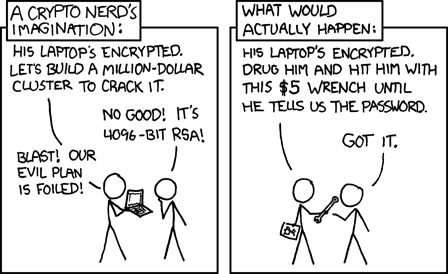
\includegraphics[width=0.7\textwidth]{crypto.png}
	
	\url{http://xkcd.com/538/}
  \end{figure}
\end{frame}





\end{document}

  